\documentclass[12pt,a4paper]{article}
\usepackage{ctex}
\usepackage{amsmath,amscd,amsbsy,amssymb,latexsym,url,bm,amsthm}
\usepackage{epsfig,graphicx,subfigure}
\usepackage{enumerate}
\usepackage{wrapfig}
\usepackage{mathrsfs,euscript}
\usepackage[usenames]{xcolor}
\usepackage{hyperref}
\usepackage[vlined,ruled,linesnumbered]{algorithm2e}
\hypersetup{colorlinks=true,linkcolor=black}

\newtheorem{theorem}{Theorem}
\newtheorem{lemma}[theorem]{Lemma}
\newtheorem{proposition}[theorem]{Proposition}
\newtheorem{corollary}[theorem]{Corollary}
\newtheorem{exercise}{Exercise}
\newtheorem*{solution}{Solution}
\newtheorem*{conclusion}{Conclusion}
\newtheorem{definition}{Definition}
\theoremstyle{definition}

\renewcommand{\thefootnote}{\fnsymbol{footnote}}

\newcommand{\postscript}[2]
 {\setlength{\epsfxsize}{#2\hsize}
  \centerline{\epsfbox{#1}}}

\renewcommand{\baselinestretch}{1.0}

\setlength{\oddsidemargin}{-0.365in}
\setlength{\evensidemargin}{-0.365in}
\setlength{\topmargin}{-0.3in}
\setlength{\headheight}{0in}
\setlength{\headsep}{0in}
\setlength{\textheight}{10.1in}
\setlength{\textwidth}{7in}
\makeatletter \renewenvironment{proof}[1][Proof] {\par\pushQED{\qed}\normalfont\topsep6\p@\@plus6\p@\relax\trivlist\item[\hskip\labelsep\bfseries#1\@addpunct{.}]\ignorespaces}{\popQED\endtrivlist\@endpefalse} \makeatother
\makeatletter
\renewenvironment{solution}[1][Solution] {\par\pushQED{\qed}\normalfont\topsep6\p@\@plus6\p@\relax\trivlist\item[\hskip\labelsep\bfseries#1\@addpunct{.}]\ignorespaces}{\popQED\endtrivlist\@endpefalse} \makeatother

\begin{document}
\noindent

%========================================================================
\noindent\framebox[\linewidth]{\shortstack[c]{
\Large{\textbf{Homework 08}}\vspace{1mm}\\
CS499-Mathematical Foundations of Computer Science, Jie Li, Spring 2020.}}
\begin{center}
\footnotesize{\color{blue}Name: ������ (Hongjie Fang)  \quad Student ID: 518030910150 \quad Email: galaxies@sjtu.edu.cn}
\end{center}
\section{Warmup Problems}
\begin{enumerate}
  \item [1. ] An eccentric collector of $2 \times n$ domino tilings pay $\$4$ for each vertical domino and $\$1$ for each horizontal domino. How many tilings are worth exactly $\$m$ by this criterion? For example, when $m = 6$ there are three solutions as follows.
      \begin{figure}[h]
      \centering
      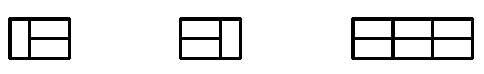
\includegraphics[width=2in]{pic1.png}\\
      \end{figure}

      \begin{solution}
      Suppose there are $T_m$ tilings worth exactly $\$m$ by this criterion. And let us focus on some small cases first.
      \begin{itemize}
      \item When $m = 0$, we know $T_0 = 1$, since there is a null tiling worth exact $\$0$ by this criterion.
      \item When $m = 1$, we know $T_1 = 0$, since there is no tiling worth exact $\$1$ by this criterion.
      \item When $m = 2$, we know $T_2 = 1$, since there is only one tiling worth exact $\$2$ by this criterion, which uses two horizontal dominos to form a $2 \times 2$ rectangle. Therefore, we have the conclusion that $T_2 = T_0$.
      \item When $m = 3$, we know $T_3 = 0$, since there is no tiling worth exact $\$3$ by this criterion.
      \end{itemize}
      Now let us see what will happen when $m \geq 4$.
      \begin{itemize}
      \item If we choose a horizontal domino, then we must choose another horizontal domino to form a $2 \times 2$ small rectangle. Therefore, we need $\$2$ in total, which leaves us $T_{m-2}$ ways to arrange the rest of our money by this criterion.
      \item If we choose a vertical domino, then we it can form a $2 \times 1$ small rectangle by itself. Therefore, we need $\$4$ in total, which leaves us $T_{m-4}$ ways to arrange the rest of our money by this criterion.
      \end{itemize}
      Therefore, we have the following recurrence (Eqn.~\eqref{eq1}).
      \begin{equation}
      T_m = T_{m-2} + T_{m-4}, \quad(m \geq 4)
      \label{eq1}
      \end{equation}
      Suppose the generating function of $T_m$ is $G(z)$, which is displayed as follows.
      \begin{displaymath}
      G(z) = \sum_{m \geq 0} T_m z^m
      \end{displaymath}
      According to the recurrence of $T_m$, we can get an equation of $G(z)$ as follows.
      \begin{displaymath}
      \begin{aligned}
      G(z) &= \sum_{m \geq 0} T_m z^m \\
           &= T_0 + T_2 z^2 + \sum_{m \geq 4} (T_{m-2} + T_{m-4}) z^m \\
           &= 1 + T_0 z^2 + T_1z^3 + \sum_{m \geq 2} T_m z^{m+2} + \sum_{m \geq 0} T_m z^{m+4} \\
           &= 1 + z^2 \sum_{m \geq 0} T_m z^m + z^4 \sum_{m \geq 0} T_m z^m \\
           &= 1 + z^2 G(z) + z^4 G(z)
      \end{aligned}
      \end{displaymath}
      Solve the simple equation, we get the closed form of $G(z)$ (Eqn.~\eqref{eq2}).
      \begin{equation}
      G(z) = \frac{1}{1 - z^2 - z^4}
      \label{eq2}
      \end{equation}

      It's a bit familiar! We know that the generating function for Fibonacci Numbers series $\{0,1,1,2,3,5,8,\cdots\}$ is
      \begin{displaymath}
      F(z) = \frac{z}{1 - z - z^2}
      \end{displaymath}
      Then there is a simple relation between $F(z)$ and $G(z)$, which is
      \begin{displaymath}
      G(z) = \frac{1}{z^2}F(z^2)
      \end{displaymath}
      Let us write the relation above in a summation form, which can shows the relation between $T_m$ and Fibonacci Numbers $F_m$ more explicitly.
      \begin{displaymath}
      \begin{aligned}
      \sum_{m \geq 0} T_m z^m &= \frac{1}{z^2} \sum_{m \geq 0} F_m (z^2)^m \\
                              &= \sum_{m \geq 2} F_m z^{2m - 2} \\
                              &= \sum_{m \geq 0} [m\textrm{ is even}] F_{\lfloor \frac{m}{2} \rfloor + 1} z^m
      \end{aligned}
      \end{displaymath}
      Therefore, we know the value of $T_m$ by referring to the corresponding term of the right-hand side. The answer of the question is as follows (Eqn.~\eqref{eq3}).
      \begin{equation}
      T_m = \left\{
      \begin{aligned}
      & 0 && \quad \quad (m\textrm{ is odd})\\
      & F_{\frac{m}{2} + 1} && \quad \quad (m\textrm{ is even})
      \end{aligned}
      \right.
      \label{eq3}
      \end{equation}
      \end{solution}

  \item [2. ] Give the generating function and the exponential generating function for the sequence
      \begin{displaymath}
      \{2,5,13,35,\cdots\} = \{2^n + 3^n\}
      \end{displaymath}
      in closed form.
      \begin{solution}
      Suppose the generating function for the sequence is $F(z)$ and the exponential generating function for the sequence is $G(z)$. It's easy to derive the closed form of generating function $F(z)$ as follows.
      \begin{displaymath}
      \begin{aligned}
      F(z) &= \sum_{n \geq 0} (2^n + 3^n) z^n \\
           &= \sum_{n \geq 0} (2z)^n + \sum_{n \geq 0} (3z)^n \\
           &= \frac{1}{1 - 2z} + \frac{1}{1 - 3z}
      \end{aligned}
      \end{displaymath}
      The derivations of exponential generating function $G(z)$'s closed form are as follows.
      \begin{displaymath}
      \begin{aligned}
      G(z) &= \sum_{n \geq 0} (2^n + 3^n) \frac{z^n}{n!} \\
           &= \sum_{n \geq 0} \frac{(2z)^n}{n!} + \sum_{n \geq 0} \frac{(3z)^n}{n!} \\
           &= e^{2z} + e^{3z}
      \end{aligned}
      \end{displaymath}
      Therefore, the generating function $F(z)$ and exponential generating function $G(z)$ is as follows (Eqn.~\eqref{eq4}).
      \begin{equation}
      F(z) = \frac{1}{1-2z} + \frac{1}{1-3z}, \quad  G(z) = e^{2z} + e^{3z}
      \label{eq4}
      \end{equation}
      \end{solution}

  \item [3. ] What is $\sum_{n \geq 0} \frac{H_n}{10^n}$ ?
      \begin{solution}
      The convergence radius of the formula above is $1$. The generating function $H(z)$ of Harmonic Numbers $H_n$ is as follows, according to Formula (7.43) in textbook.
      \begin{displaymath}
      H(z) = \sum_{n \geq 0} H_n z^n = \frac{1}{1-z} \ln{\frac{1}{1-z}}
      \end{displaymath}
      Since $\frac{1}{10}$ is within the convergence radius, we can set $z = \frac{1}{10}$ in the formula above, and we can simplify the given formula.
      \begin{displaymath}
      \begin{aligned}
      \sum_{n \geq 0} \frac{H_n}{10^n} &= \sum_{n \geq 0} H_n \left(\frac{1}{10}\right)^n \\
                                 &= \frac{1}{1-\frac{1}{10}} \ln{\frac{1}{1-\frac{1}{10}}} \\
                                 &= \frac{10}{9} \ln{\frac{10}{9}}.
      \end{aligned}
      \end{displaymath}
      Therefore, the value of the given formula is $\frac{10}{9} \ln{\frac{10}{9}}$.
      \end{solution}
\end{enumerate}
\section{Basic Problems}
\begin{enumerate}
  \item [7. ] Solve the recurrence
  \begin{displaymath}
  \begin{aligned}
  & g_0 = 1 \\
  & g_n = g_{n-1} + 2g_{n-2} + \cdots + ng_0, \quad \textrm{for } n > 0
  \end{aligned}
  \end{displaymath}
      \begin{solution}
      Suppose the generating function of $\{g_0, g_1, g_2, \cdots\}$ is $G(z)$, which means
      \begin{displaymath}
      G(z) = \sum_{n \geq 0} g_n z^n
      \end{displaymath}
      According to the textbook, the the generating function $F(z)$ for sequence $\{0,1,2,3,4,\cdots\}$ is
      \begin{displaymath}
      F(z) = \frac{z}{(1-z)^2}
      \end{displaymath}

      It's easy to find out that the recurrence has a form of convolution between $\{g_n\}$ and $\{0,1,2,3,4,\cdots\}$. Therefore, we can derive a equation of $G(z)$ as follows.
      \begin{displaymath}
      \begin{aligned}
      G(z) &= \sum_{n \geq 0} g_n z^n \\
           &= g_0 + \sum_{n \geq 1}\left(\sum_{k = 0}^n k g_{n-k} \right)\\
           &= g_0 + \sum_{n \geq 0}\left(\sum_{k = 0}^n k g_{n-k} \right)\\
           &= 1 + F(z) \cdot G(z)
      \end{aligned}
      \end{displaymath}
      Solve the equation, we can get the closed form of $G(z)$ as follows (Eqn.~\eqref{eq5}).
      \begin{equation}
      G(z) = \frac{1}{1 - F(z)} = \frac{1}{1 - \frac{z}{(1-z)^2}} = \frac{z^2 - 2z + 1}{z^2 - 3z + 1} = 1 + \frac{z}{z^2 - 3z + 1}
      \label{eq5}
      \end{equation}
      This closed form is very similar to Formula (7.24) in textbook, which is displayed as follows.
      \begin{displaymath}
      \sum_{n \geq 0} F_{2n} z^n = \frac{z}{1 - 3z + z^2}
      \end{displaymath}
      Therefore, the generating function of $G(z)$ can be written as follows.
      \begin{displaymath}
      G(z) = 1 + \sum_{n \geq 0} F_{2n} z^n
      \end{displaymath}
      Hence, we have the following conclusion (Eqn.~\eqref{eq6}).
      \begin{equation}
      g_n = F_{2n} + [n = 0]
      \label{eq6}
      \end{equation}
      \end{solution}

  \item [8. ] What is the value of the following formula?
  \begin{displaymath}
  [z^n]\frac{(\ln{(1-z)})^2}{(1-z)^{m+1}}
  \end{displaymath}
      \begin{solution}
        Table 335 in the textbook tells us the following property.
        \begin{displaymath}
        \sum_{n\geq 0} \binom{c+n-1}{n} z^n = \frac{1}{(1-z)^c}
        \end{displaymath}
        Set $x = c-1$ in the formula above, and differentiate twice with respect to $x$, we can make the following derivations.
        \begin{displaymath}
        \begin{aligned}
        & \quad \frac{\mathrm{d}^2}{\mathrm{d}x^2} \sum_{n\geq 0} \binom{x+n}{n} z^n = \frac{\mathrm{d}^2}{\mathrm{d}x^2}\frac{1}{(1-z)^{x+1}}\\
        \Longrightarrow & \quad \frac{\mathrm{d}^2}{\mathrm{d}x^2} \sum_{n\geq 0} \frac{(x+n)^{\underline{n}}}{n!} z^n = \frac{(\ln{(1-z)})^2}{(1-z)^{x+1}}\\
        \Longrightarrow & \quad \frac{\mathrm{d}}{\mathrm{d}x} \sum_{n\geq 0} \frac{(x+n)^{\underline{n}}}{n!}(H_{x+n} - H_x) z^n = \frac{(\ln{(1-z)})^2}{(1-z)^{x+1}}\\
        \Longrightarrow & \quad \sum_{n\geq 0} \frac{(x+n)^{\underline{n}}}{n!}((H_{x+n} - H_x)^2 - (H_{x+n}^{(2)} - H_x^{(2)})) z^n = \frac{(\ln{(1-z)})^2}{(1-z)^{x+1}}\\
        \Longrightarrow & \quad \sum_{n\geq 0} \binom{x+n}{n} ((H_{x+n} - H_x)^2 - (H_{x+n}^{(2)} - H_x^{(2)})) z^n = \frac{(\ln{(1-z)})^2}{(1-z)^{x+1}}\\
        \end{aligned}
        \end{displaymath}
        where, $H_x^{(2)}$ stands for
        \begin{displaymath}
        \sum_{1 \leq k \leq x} \frac{1}{k^2}
        \end{displaymath}
        Set $x = m$, then the value of the formula is as follows (Eqn.~\eqref{eq7})
        \begin{equation}
        [z^n]\frac{(\ln{(1-z)})^2}{(1-z)^{m+1}} = \binom{m+n}{n} ((H_{m+n} - H_m)^2 - (H_{m+n}^{(2)} - H_m^{(2)}))
        \label{eq7}
        \end{equation}
      \end{solution}

  \item [9. ] Use the result of the previous exercise to evaluate $\sum_{k=0}^n H_k H_{n-k}$.
      \begin{solution}
      According to (7.43) in textbook, we know that the generating function $H(z)$ for Harmonic Numbers $H_n$ is as follows.
      \begin{displaymath}
      H(z) = \sum_{n \geq 0} H_n z^n = \frac{1}{1-z} \ln{\frac{1}{1-z}}
      \end{displaymath}
      Suppose the generating function for the number series $\{ \sum_{k=0}^n H_k H_{n-k} \}$ is $H^*(z)$, then it's obvious that $H^*(z) = H^2(z)$ since $\sum_{k=0}^n H_k H_{n-k}$ is a convolution form. Hence,
      \begin{displaymath}
      H^*(z) = \frac{(\ln{(1-z)})^2}{(1-z)^2}
      \end{displaymath}
      Therefore, using the result of the last exercise, we can get the value of the given formula as follows.
      \begin{displaymath}
      \begin{aligned}
      \sum_{k=0}^n H_k H_{n-k} &= [z^n] H^*(z)\\
                               &= [z^n] \frac{(\ln{(1-z)})^2}{(1-z)^2}\\
                               &= \binom{1+n}{n} ((H_{1+n} - H_1)^2 - (H_{1+n}^{(2)} - H_1^{(2)})) \\
                               &= (n+1) \left(\left(H_n + \frac{1}{n+1} - 1\right)^2 - H_n^{(2)} - \frac{1}{(n+1)^2} + 1\right) \\
                               &= (n+1) \left((H_n-1)^2 + 2\frac{H_n - 1}{n+1} - H_n^{(2)} + 1\right) \\
                               &= (n+1) \left(H_n^2 - 2H_n + 2\frac{H_n - 1}{n+1} - H_n^{(2)}+ 2\right) \\
                               &= (n+1) (H_n^2 - H_n^{(2)}) - 2(H_n-1)(n+1) + 2(H_n-1) \\
                               &= (n+1) (H_n^2 - H_n^{(2)}) - 2n(H_n-1)
      \end{aligned}
      \end{displaymath}
      Hence, the result of the given formula is
      \begin{displaymath}
      (n+1) (H_n^2 - H_n^{(2)}) - 2n(H_n-1)
      \end{displaymath}
      \end{solution}
\end{enumerate}
\section{Homework Exercises}
\begin{enumerate}
  \item [21. ] \textbf{(Bonus Problem)} A robber holds up a bank and demands $\$500$ in tens and twenties. He also demands to know the number of ways in which the cashier can give him the money. Find a generating function $G(z)$ for which this number is $[z^{500}]G(z)$, and a more compact generating function $\check{G}(z)$ for which this number is $[z^{50}]\check{G}(z)$. Determine the required number of ways by (a) using partial fractions; (b) using a method like (7.39).
      \begin{solution}
      The generating function for only using $\$10$ is $\frac{1}{1 - z^{10}}$, and similarly, the generating function for only using $\$20$ is $\frac{1}{1-z^{20}}$. Therefore, the generating function $G(z)$ for using $\$10$ and $\$20$ is as follows (Eqn.~\eqref{eq8})
      \begin{equation}
      G(z) = \frac{1}{1-z^{10}} \cdot \frac{1}{1-z^{20}}
      \label{eq8}
      \end{equation}
      According to the definition of $\check{G}(z)$, we know that
      \begin{displaymath}
      \check{G}(z^{10}) = G(z) \quad \Longrightarrow \quad \check{G}(z) = \frac{1}{(1 - z)(1 - z^2)}
      \end{displaymath}
      \begin{enumerate}
      \item [a. ] \textbf{(Partial Fractions Decomposition)} Suppose $\check{G}(z)$ can be decomposed as follows.
      \begin{displaymath}
      \check{G}(z) = \frac{1}{(1 - z)(1 - z^2)} = \frac{1}{(1-z)^2(1+z)} = \frac{A}{1+z} + \frac{B}{1-z} + \frac{C}{(1-z)^2}
      \end{displaymath}
      where $A, B, C$ are const numbers. Then we can simplify the formula above.
      \begin{displaymath}
      \begin{aligned}
      \check{G}(z) &= \frac{A(1-z)^2 + B(1-z^2) + C(1+z)}{(1-z)^2(1+z)} \\
                   &= \frac{(A - B)z^2 + (C - 2A)z + A + B + C}{(1-z)^2(1+z)}
      \end{aligned}
      \end{displaymath}
      According to the previous result, the numerator should be $1$. Thus,
      \begin{displaymath}
      \left\{
      \begin{aligned}
      & A - B = 0 \\
      & C - 2A = 0 \\
      & A + B + C = 1 \\
      \end{aligned}
      \right.
      \end{displaymath}
      Solve the equations then we can get $A = \frac{1}{4}, B = \frac{1}{4}, C = \frac{1}{2}$. Hence we can rewrite $\check{G}(z)$ as follows (Eqn.~\eqref{eq9}).
      \begin{equation}
      \begin{aligned}
      \check{G}(z) & = \frac{1}{4} \cdot \frac{1}{1+z} + \frac{1}{4} \cdot \frac{1}{1-z} + \frac{1}{2} \cdot \frac{1}{(1-z)^2} \\
                   & = \frac{1}{4} \sum_{n \geq 0} (-z)^n + \frac{1}{4} \sum_{n \geq 0} z^n + \frac{1}{2} \sum_{n \geq 0} (n+1)z^n \\
                   & = \sum_{n \geq 0} \frac{1}{4}(2n + 3 + (-1)^n) z^n
      \end{aligned}
      \label{eq9}
      \end{equation}
      Therefore,
      \begin{equation}
      [z^n]\check{G}(z) = \frac{1}{4}(2n + 3 + (-1)^n)
      \label{eq10}
      \end{equation}
      Plug $n = 50$ into the Equation \eqref{eq10}, and we get $[z^{50}]\check{G}(z) = 26$. So there are $26$ ways in which the cashier can give the robber the money.
      \item [b. ] \textbf{(Method like (7.39))} We can rewrite $\check{G}(z)$ as follows (Eqn.~\eqref{eq11}).
      \begin{equation}
      \begin{aligned}
      \check{G}(z) &= \frac{1 + z}{(1 - z^2)^2} \\
                   &= (1+z) \sum_{n \geq 0}(n+1)(z^2)^n \\
                   &= \sum_{n \geq 0} (n+1) z^{2n} + \sum_{n \geq 0} (n+1) z^{2n+1} \\
                   &= \sum_{n \geq 0} \left(\left\lfloor \frac{n}{2} \right\rfloor + 1\right)z^n
      \end{aligned}
      \label{eq11}
      \end{equation}
      Therefore,
      \begin{equation}
      [z^n]\check{G}(z) = \left\lfloor \frac{n}{2} \right\rfloor + 1
      \label{eq12}
      \end{equation}
      Plug $n = 50$ into the Equation \eqref{eq12}, and we get $[z^{50}]\check{G}(z) = 26$. So there are $26$ ways in which the cashier can give the robber the money.

      \end{enumerate}
      \end{solution}
\end{enumerate}
%=================== =====================================================
\end{document}
